\documentclass{beamer}
\def\presentationtype{0}
\def\corsodilaurea{Ingegneria Informatica e dell'Automazione Industriale}
\def\insegnamento{Ottimizzazione}
\def\nolezione{8}
\def\titolo{Il metodo del simplesso -- Il ``tableau'' e l'operazione ``pivot''}
\def\noattivita{1}

\def\argomenti{Programmazione Lineare}
\def\obiettivilezione{Definire il ``tableau'' e l'operazione ``pivot'' per poter sviluppare metodo del simplesso primale}
\def\nucleotematico{Richiami}
\def\contenuto{Programmazione lineare}


\usepackage[italian]{babel}
%
% Hyperref info for PDF
%
\usepackage{hyperref}
\hypersetup{%
%pdfpagemode=FullScreen,
pdfpagemode=FullScreen,
pdfstartview=Fit,
pdfsubject={\argomenti},
pdfkeywords={\insegnamento,\titolo}
}

\definecolor{ecampus@engred}{RGB}{227,28,23}
\setbeamercolor{normal text}{fg=black,bg=}
\setbeamercolor{alerted text}{fg=red}
\setbeamercolor{example text}{fg=green!50!black}
\setbeamercolor{structure}{fg=ecampus@engred,bg=}
\usetheme{default}
\useinnertheme{rounded}%{circles}
\setbeamertemplate{blocks}[default]
\setbeamercolor{block title}{bg=}
\setbeamercolor{block body}{bg=}

\ifnum\presentationtype>0 {\setbeamertemplate{enumerate item}{Es. \nolezione.\presentationtype.\arabic{enumi})}} \fi

%\setbeamertemplate{frametitle continuation}[from second][(cont'd)]
\usefonttheme[stillsansseriftext,stillsansserifsmall]{serif}
\setbeamertemplate{headline}{%
\leavevmode%
   \hspace*{4.75cm}
   \scalebox{0.90}{%
    \begin{minipage}{\linewidth}%
      \tiny
 	\begin{tabular}{ll}
	  \\
% 	  \textcolor{gray}{Classe}					& \corsodilaurea\\
%	  \textcolor{gray}{Argomento:}					& \insegnamento\\
%	  \textcolor{gray}{Lezione n}:							& \nolezione \\
	  \textcolor{gray}{Titolo:}			& \titolo \\
	  \textcolor{gray}{Attivit\`a}:		& 	  \ifnum\presentationtype=0 {Lezione \nolezione} \else {Sessione di studio \nolezione.\presentationtype} \fi
	\end{tabular}%
    \end{minipage}%
   }%
}
\setbeamertemplate{footline}[text line]{%
  \begin{minipage}{\linewidth}%
    \hfill\insertpagenumber%
%    
    \begin{center}%
      \rule{\linewidth}{0.4pt}
    \end{center}
    \vspace*{-0.65cm}
    \begin{center}%
      \scalebox{0.55}{%
	\begin{minipage}{\linewidth}%
	  \begin{center}%
	    {\tiny
	    \copyright \ 2022 Gionata Massi - \color{blue}{\href{mailto:gionata.massi@savoiabenincasa.it}{gionata.massi@savoiabenincasa.it}}\\
	    \phantom{XXX}}
	  \end{center}
	\end{minipage}%
      }%
    \end{center}%
%
  \end{minipage}%
  }
\setbeamertemplate{navigation symbols}{}

%% Save up on ink for the 4-up handouts
\mode<handout>{%
  \pgfpagesuselayout{4 on 1}[a4paper, landscape, border shrink=10mm]
  \pgfpageslogicalpageoptions{1}{border code=\pgfstroke}
  \pgfpageslogicalpageoptions{2}{border code=\pgfstroke}
  \pgfpageslogicalpageoptions{3}{border code=\pgfstroke}
  \pgfpageslogicalpageoptions{4}{border code=\pgfstroke}
}

\mode<presentation>{\AtBeginSection{%
  \begin{frame}
    \frametitle{Piano della presentazione}
    \tableofcontents[currentsection]
  \end{frame}}
}

\usepackage{microtype}
\usepackage[utf8]{inputenc}
\usepackage[T1]{fontenc}
%\usepackage[osfss]{libertine}
\usepackage{palatino}
\usepackage[scaled=.77]{beramono}
\usepackage{booktabs}
% \usepackage{attachfile}

% Toglie l'enorme spazione prima di description
%\setbeamersize{description width=0pt}

\usepackage{tikz}
\usetikzlibrary{decorations,arrows,shapes,backgrounds,matrix,positioning}
\usepackage{multirow}
\usepackage{verbatim}
\usepackage{eurosym}
\usepackage{pgfpages}

\usepackage{zref-savepos}
\newcounter{restofframe}
\newsavebox{\restofframebox}
\newlength{\mylowermargin}
\setlength{\mylowermargin}{2pt}

\newenvironment{restofframe}{%
    \par%\centering
    \stepcounter{restofframe}%
    \zsavepos{restofframe-\arabic{restofframe}-begin}%
    \begin{lrbox}{\restofframebox}%
}{%
    \end{lrbox}%
    \setkeys{Gin}{keepaspectratio}%
    \raisebox{\dimexpr-\height+\ht\strutbox\relax}[0pt][0pt]{%
    \resizebox*{!}{\dimexpr\zposy{restofframe-\arabic{restofframe}-begin}sp-\zposy{restofframe-\arabic{restofframe}-end}sp-\mylowermargin\relax}%
        {\usebox{\restofframebox}}%
    }%
    \vskip0pt plus 1filll\relax
    \mbox{\zsavepos{restofframe-\arabic{restofframe}-end}}%
    \par
}

\title{\titolo}
\author{Gionata Massi}
\date{\today}

\setbeamercolor*{frametitle}{fg=black}
\setbeamercolor*{title}{fg=black}
\setbeamerfont{frametitle}{shape=\scshape,family=\rmfamily,size=\large,series=\bfseries}

\setbeamersize{}
\makeatletter
\newcommand\thefontsize[1]{{#1 The current font size is: \f@size pt\par}}
\makeatother

\tikzstyle{nicebox}=[draw=gray!100, fill=blue!10, very thick,
rounded corners, rectangle, inner sep=4pt, inner ysep=16pt]
\tikzstyle{niceboxtitle}=[draw=gray!100, fill=white, text=black,
rounded corners, very thick, rectangle]
\newcommand\nicebox[2]{
{\centering
\begin{tikzpicture}
\node [nicebox](box){
\begin{minipage}{0.95\textwidth}\centering
\begin{minipage}{0.95\textwidth}
#2
\end{minipage}\end{minipage}};
\node[niceboxtitle, right=10pt] at (box.north west)
{\small\textbf{#1}};
\end{tikzpicture}\par}
}

\tikzstyle{modelbox}=[draw=structure!100, fill=white!50, very thick,
rounded corners, rectangle, inner sep=4pt, inner ysep=16pt, text=blue!50!black]
\tikzstyle{modelboxtitle}=[draw=structure!100, fill=white!50, text=blue!50!black,
rounded corners, very thick, rectangle]
\newcommand\modelbox[2]{
{\centering
\begin{tikzpicture}
\node [modelbox](box){
\begin{minipage}{0.95\textwidth}\centering
\begin{minipage}{0.95\textwidth}
#2
\end{minipage}\end{minipage}};
\node[modelboxtitle, right=10pt] at (box.north west)
{\small\textbf{\mbox{#1}}};
\end{tikzpicture}\par}
}

% % %
% Tipi di sessioni di studio
% % %
\def\domande{Domande}
\def\approfondimenti{Approfondimenti}
\def\esercizi{Esercizi}
\def\esempi{Esempi svolti}
\def\relazioni{Relazioni}
\def\attivitapratica{Attivit\`a pratica}
% % %

\newcommand{\generatitolo}{ %
\begin{frame}[plain]
\pdfbookmark{\ifnum\presentationtype=0 {Lezione \nolezione} \else {Sessione di studio \nolezione.\presentationtype} \fi}{\ifnum\presentationtype=0 {Lezione \nolezione} \else {Sessione di studio \nolezione.\presentationtype} \fi}
\noindent\hspace*{3.715cm}
   \scalebox{0.90}{%
    \begin{minipage}{\linewidth}%
      \tiny
 	\begin{tabular}{ll}
	  \\
% 	  \textcolor{gray}{Classe}					& \corsodilaurea\\
%	  \textcolor{gray}{Argomento:}					& \insegnamento\\
%	  \textcolor{gray}{Lezione n}:							& \nolezione \\
	  \textcolor{gray}{Titolo:}			& \titolo \\
	  \textcolor{gray}{Attivit\`a}:		& 	  \ifnum\presentationtype=0 {Lezione \nolezione} \else {Sessione di studio \nolezione.\presentationtype} \fi
	\end{tabular}%
    \end{minipage}%
   }%
   
  \begin{center}
    \large{\textbf{\insegnamento}}
  \end{center}

  \vspace*{0.5cm}
  
  \begin{center}
    \huge{\titolo}
  \end{center}
  
  \begin{center}
	  \ifnum\presentationtype=0
	    {Lezione n$^{\circ}$ \nolezione}
	  \else
	    {Sessione di studio n$^{\circ}$ \nolezione .\presentationtype}
	  \fi
  \end{center}
  
  \vspace*{0.5cm}

  \begin{center}
    \large{\textsl{Gionata Massi}}\\
    \scriptsize\color{blue}{<\href{mailto:gionata.massi@savoiabenincasa.it}{gionata.massi@savoiabenincasa.it}>}
  \end{center}
  
  \newcounter{pageleft}
  \zsaveposy{pageleft}
  \vspace*{\dimexpr\zposy{pageleft}sp-1.67cm}

  \begin{minipage}{\linewidth}%
   \hfill\phantom{\insertpagenumber}%

  \begin{center}%
      \rule{\linewidth}{0.4pt}
    \end{center}
    
    \vspace*{-0.95cm}
    
    \begin{center}%
      \scalebox{0.55}{%
	\begin{minipage}{\linewidth}%
	  %\begin{center}%
	  %  \tiny
	  %  \copyright \ 2022 Gionata Massi - \color{blue}{\href{mailto:gionata.massi@savoiabenincasa.it}{gionata.massi@savoiabenincasa.it}}\\
	  %  \color{blue}{\href{mailto:gionata.massi@savoiabenincasa.it}{gionata.massi@savoiabenincasa.it}}\\
	  %  \phantom{XXX}
	  %\end{center}
	\end{minipage}%
      }%
    \end{center}%
     \phantom{XXX}
%
  \end{minipage}%

\end{frame}
}

\renewcommand{\vec}{\mathbf}
\newcommand{\matr}{\mathbf}

\uselanguage{italian}
\languagepath{italian}
\deftranslation[to=italian]{Theorem}{Teorema}
\deftranslation[to=italian]{theorem}{teorema}
\deftranslation[to=italian]{Definition}{Definizione}
\deftranslation[to=italian]{definition}{definizione}
\deftranslation[to=italian]{Corollary}{Corollario}
\deftranslation[to=italian]{corollary}{corollario}

\let\definition\relax
\let\enddefinition\relax

%\theoremstyle{example}
\newtheorem{definition}[theorem]{\translate{Definition}}

\def\fieldN{\mathbb{N}}
\def\fieldR{\mathbb{R}}
\def\fieldZ{\mathbb{Z}}

\def\matrA{\matr{A}}
\def\vecB{\vec{b}}
\def\vecC{\vec{c}}
\def\vecX{\vec{x}}

\usepackage{cancel}
\usepackage{bookmark}

% tkiz ball item
\newcommand*\circled[1]{\raisebox{2.5pt}{\tikz[baseline=(char.base)]{
            \node[circle,ball color=purple, shade, 
 color=white,inner sep=1.2pt] (char) {\tiny #1};}}}

% tkiz rounded item
\newcommand*\rounded[1]{\tikz[baseline=(char.base)]{
            \node[draw=none,ball color=purple, shade, 
 color=white, rounded corners=3.5pt, inner sep=2.5pt] (char) {\scriptsize #1};}}

 \usepackage{etoolbox}
\makeatletter
\apptocmd{\beamer@@frametitle}{\write\@auxout{\string\@writefile{frm}{\string\frametitleentry{\the\c@framenumber}{#1}{#2}}}}{}{}
\newcommand*{\frametitleentry}[3]{\@namedef{frametitleshort#1}{#2}\@namedef{frametitle#1}{#3}}
\AtEndDocument{\if@filesw\newwrite\tf@frm\immediate\openout\tf@frm\jobname.frm\relax\fi}
\@input{\jobname.frm}
\makeatother
 
%\usebackgroundtemplate{
\includegraphics[width=\paperwidth]{../img/sfondo_ecampus.png}}

\usepackage{listings}
% Extension for listings package
\lstdefinelanguage{ampl}{
  % See AMPL book (1993 edition), Appendix A
  morekeywords={%
    % Table A.1
    % Excluding symbols and "not X", where X (and not) are keywords
    if, then, else, or,  exists, forall,  and, in, within, 
    not, union, diff, symdiff, inter, cross, setof, by, 
    % Skipping: less,  sum, prod, min, max, div, mod,
    % Skipping built-in functions (Tables A-2 and A-3)
    % Section A.5 -- Declarations of model entities (subject to ->
    % subject, to)
    set, param, var, arc, minimize, maximize, subject, to, node,
    % Section A.6 -- Set declarations (not repeating set or within)
    dimen, default, card, ordered, by, reversed, circular,
    % Section A.7 -- Parameter declarations (not repeating in, default)
    param, binary, integer, symbolic, check, Infinity
    % Section A.8 -- Variable declarations
    var,  coeff, cover, obj,
    % Section A.13 -- Command language
    % Skipping most commands!
    include, model, data, let, objective, drop, restore, solve,
    solution, quit, end, option, reset, update, commands,
    % A.14 -- Imported functions
    function, pipe, 
    % A.17 synonyms for previously-defined keywords
    coef, difference, dimen, dimension, intersect, intersection, s.t., 
    % 
    % must be defined somewhere ...
    for, while, repeat, break,
    % NEW language features (http://www.ampl.com/NEW/newlang.html)
    % Grouped by page
    purge, problem, redeclare, xref,
    complements, 
    table, IN, OUT, INOUT, read, write, 
    expand,
    for, commands, repeat, until, while, break, continue,
  },
  sensitive=true,
  comment=[l]{\#},
  morecomment=[s]{/*}{*/},
  string=[b]",
  morestring=[b]',
}[keywords,comments,strings]

\definecolor{comment_c}{RGB}{60,128,49}
\definecolor{rowname_c}{RGB}{128,60,49}
\definecolor{reserved_c}{RGB}{49,60,128}

\lstset{
	language=ampl,%
	commentstyle=\color{comment_c},%
	backgroundcolor=\color{blue!15},%
    basicstyle=\small\ttfamily,%
    %emph={s.t.},emphstyle={\bfseries},%
    otherkeywords={s.t.},%
    numbers=left, numberstyle=\tiny, stepnumber=1, numbersep=5pt,%
}

\definecolor{col_set}{RGB}{128,0,0}
\definecolor{col_par}{RGB}{91,0,91}
\definecolor{col_idx}{RGB}{0,91,91}
\definecolor{col_var}{RGB}{0,0,128}

\def\insieme{%1}{\rm \textcolor{col_set}{%1}}}


\begin{document}

\generatitolo

\section{Risolvere un Programma Lineare}

\begin{frame}[allowframebreaks]{Il metodo del Simplesso}

\begin{itemize}
\item Il metodo del simplesso primale \`e un algoritmo per la risoluzione algebrica di problemi di P.L. espressi in forma canonica forte.

\item \`E il metodo proposto da George Dantzig nel 1947
per la risoluzione dei problemi generali di P.L.
Per anni \`e stato anche l'unico algoritmo disponibile.

\item Rimane un metodo tra i pi\`u utilizzati per la soluzione di problemi di P.L. nonostante attualmente siano disponibili altri algoritmi.

\item Pu\`o essere utilizzato, insieme ad altre tecniche, nella risoluzione dei problemi di P.L.I.

\item Permette di effettuare agevolmente l'analisi di post-ottimalit\`a.

\item  Esistono molti pacchetti software che lo implementano, sia gratuiti che commerciali.
\end{itemize}
\end{frame}

\begin{frame}[allowframebreaks]{Le possibili soluzioni}
Un problema di P.L. soddisfa sempre uno dei tre casi seguenti:

\begin{enumerate}
\item il problema \`e inammissibile: la regione ammissibile \`e vuota;

\item il problema \`e illimitato: \`e possibile trovare delle soluzioni ammissibili facendo crescere a piacere il valore di una o pi\`u variabili decisionali in modo che la funzione obiettivo diminuisca (o aumenti per problemi di massimo) a piacere;

\item il problema ammette soluzione ottima: esiste almeno una soluzione ammissibile che minimizza (massimizza) il valore della funzione obiettivo. Tale valore \`e limitato.
\end{enumerate}	

\begin{itemize}
\item   Risolvere un problema di P.L. significa 
  riconoscere il verificarsi di uno dei tre casi

\item   se \`e verificato il caso 3, fornire
\begin{itemize}
  \item il valore assunto all'ottimo dalle variabili decisionali (il vettore $\vecX^\star$)
  \item il valore assunto all'ottimo dalla funzione obiettivo ($z^\star$)
\end{itemize}
\end{itemize}
\end{frame}

\section{Matrice tableau}

\begin{frame}{Matrice tableau}
\begin{columns}
\begin{column}{0.7\textwidth}
{\small %
\begin{itemize}
\item Il problema di P.L. in forma canonica pu\`o essere
	rappresentato in una tabella di $m+1$ righe ed $n+1$
	colonne
	
\item La tabella $\matr{M}$ \`e una matrice, detta 
	\emph{matrice tableau}.

\item Rappresenta le equazioni del problema di
   programmazione lineare in modo compatto.

\item  Si noti che in alto a sinistra si \`e posto $-d$
che e i termini noti sono stati spostati sulla sinistra.
\end{itemize} %
}
\end{column}
\begin{column}{0.3\textwidth}
{\tiny
\centering\fbox{
\begin{minipage}{0.5\textwidth}
$\min z = \vecC^T x + d$
$$\begin{cases}
\matrA \vecX = \vecB\\
\vecX \geq \vec{0}
\end{cases}$$
\end{minipage}
}

\vfill

%$$\bordermatrix{
%        &  -z   & x_{1}    &  x_{2}	&\cdots&x_{n} \cr
%   f.o.\   &  -d      &  c_1       & c_2 & \cdots&c_{n} \cr
%	1    &  b_{1}& a_{11} & a_{12} &\cdots&a_{1n} \cr
%    2    & b_{2} & a_{21} & a_{22} &\cdots &a_{2n} \cr
%\vdots & \vdots &\vdots &\vdots &\ddots &\vdots \cr
%	m    &  b_{m}& a_{m1} & a_{m2}    &\cdots&a_{mn} \cr
%}$$
%
%\vfill

\begin{center}
\begin{tabular}{|c|p{0.2\textwidth}|}
\hline
$-d$ & \multicolumn{1}{|c|}{\phantom{\LARGE{X}}$\vecC^T$\phantom{\LARGE{X}}}\\
\hline
$\vecB$ & \multicolumn{1}{|c|}{\phantom{\LARGE{X}}$\matrA$\phantom{\LARGE{X}}}\\
\hline
\end{tabular}
\end{center}

}
\end{column}
\end{columns}
\end{frame}

\begin{frame}[fragile]{La matrice tableau di un PL in forma canonica}
\centering
\begin{tikzpicture}
{\scriptsize
\node[
  row 1/.style=gray,
  row 2/.style=blue,
  column 1/.style=gray,
  column 2/.style=red,
  row 2 column 1/.style={gray},
  cell/.style=rectangle,
  text height=2ex,
  text width=1.5em,
  align=center,
  column  9/.style={text width=2em},
  column 10/.style={text width=2em},
  column 12/.style={text width=2em},
  column 14/.style={text width=2em},
  matrix of math nodes] (M)
{
&0&1&2&\cdots&k&\cdots&p&s_1&s_2&\cdots&s_h&\cdots&s_m\\
0 & -d & c_1 & c_2 & \cdots & c_k & \cdots & c_p & \alt<1-2>{c_{s_1}}{0} &  \alt<1-2>{c_{s_2}}{0} & \cdots &  \alt<1-2>{c_{s_h}}{0} & \cdots &  \alt<1-2>{c_{s_m}}{0}\\
1& b_1 &  a_{11} &  a_{12} &  \cdots &  a_{1k} &  \cdots &  a_{1{p}}&  1 &  0 & \cdots&0 & \cdots&0\\
2& b_2 &  a_{21} &  a_{22} &  \cdots &  a_{2k} &  \cdots &  a_{2{p}}  &  0 & 1 &  \cdots & 0 & \cdots&0\\
\vdots & \vdots &  \vdots &  \vdots &  \vdots &  \ddots &  \vdots &  \ddots &  \vdots &  \vdots &\ddots  & \vdots & \cdots&0\\
h& b_h &  a_{h1} &  a_{h2} &  \cdots & a_{hk} &  \cdots &  a_{h{p}} &  0 & 0 & \cdots & 1 & \cdots&0\\
\vdots& \vdots &  \vdots &  \vdots &  \vdots &  \ddots &  \vdots &  \ddots &\vdots & \vdots  & \vdots & \vdots & \ddots&0\\
m& b_m &  a_{m1} &  a_{m2} &  \cdots &  a_{mk} &  \cdots &  a_{m{p}}&  0 &  0 & \cdots&0& \cdots & 1\\
};
% separatore verticale
\draw[dashed] (M-2-3.north west) -- (M-8-3.south west);
% separatore orizzontale
\draw[dashed] (M-3-1.north east) -- (M-3-14.north east);
% riquadro
\draw(M-2-2.north west) -- (M-2-14.north east) -- (M-8-14.south east) -- (M-8-2.south west) -- cycle;
% A_s: 3--8: 9--14
\uncover<2->{
\fill[red!50,fill opacity=0.5,thick,draw=red!60!black]  (M-3-9.north west) rectangle (M-8-14.south east);
\node[red!40!black, below = of M-8-11.north east,draw=red!40,thick] (as) {$\alpha)\ \mathbf{A}_S = \mathbf{I}_m$};
\draw[->,red!60,thick] (as) to (M-5-11.east);
}
% c_s: 2: 9--12
\onslide<3->{
\fill[green!50,fill opacity=0.5,thick,draw=green!60!black]  (M-2-9.north west) rectangle (M-2-14.south east);
\node[green!40!black, above = of M-2-11.south east,draw=green!40,thick] (cs) {$\beta)\ \mathbf{c}_S = \mathbf{0}$};
\draw[->,green!60,thick] (cs) to (M-2-11.east);
}
% b: 3--8: 2
\uncover<4->{
\fill[blue!50,fill opacity=0.5,thick,draw=blue!60!black]  (M-3-2.north west) rectangle (M-8-2.south east);
\node[blue!40!black, below = of M-8-2.north,draw=blue!40,thick] (b) {$\gamma\ \mathbf{b} \geq \mathbf{0}$};
\draw[->,blue!60,thick] (b) to [out=180,in=180] (M-5-2);
}
}
\end{tikzpicture}
%sono fragile: lasciami uno spazio vuoto

\end{frame}

\section{Pivot}

\begin{frame}[allowframebreaks]{Operazione ``pivot''}

L'operazione di ``pivot'' in posizione $(h, k )$,
con $h$ e $k$ diversi da 0,
\`e un'operazione sulla matrice tableau definita
quando $a_{hk} \neq 0$ e consiste nei seguenti passi:

\begin{itemize}
\item si dividono tutti gli elementi della riga $h$ per $a_{hk}$;

\item si sottraggono opportuni multipli della nuova riga $h$
	ottenuta al passo precedente a tutte le altre righe in modo
	tale che tutti gli elementi della colonna $k$, ad eccezione
	di quello in posizione $(h, k )$, diventino nulli.
\end{itemize}

\framebreak

Consideriamo l'operazione solo sulle matrici in forma canonica e un elemento pivot non nullo in una colonna fuori  base.
Il significato dell'operazione di pivot \`e il seguente:

\begin{itemize}
\item si risolve l'equazione $h$ rispetto a $x_k$;

\item si usa l'equazione $h$ per eliminare la variabile
	$x_k$ dalle altre equazioni di vincolo e dalla funzione
	obiettivo.
\end{itemize}

L'operazione di ``pivot'' in posizione $(h, k )$, con $h$ e $k$
diversi da 0, corrisponde a far entrare in base la variabile
fuori base $x_k$ e a far uscire dalla base la variabile $x_{s_h}$
in posizione $h$-esima nella sequenza di base.

\begin{center}
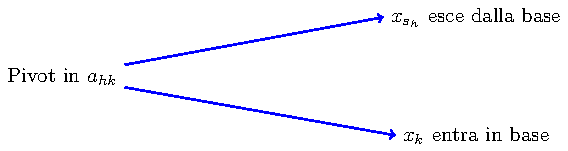
\includegraphics{img/pivot_entra_esce}
\end{center}

\begin{itemize}
\item L'operazione di pivot corrisponde al calcolo algebrico di una
nuova soluzione di base

\item A seguito dell'operazione di pivot in $(h, k)$ la matrice tableau
e la sequenza degli indici di base cambiano

\item L'elemento di pivot $a_{hk}$  \`e indicato da una circonferenza.
La variabile entrante in base $x_k$ \`e indicata da una freccia
verso il basso posta al di sopra della colonna $k$; la variabile
uscente dalla base $x_{s_h}$ \`e indicata da una freccia verso
l'alto sopra la colonna $s_h$
\end{itemize}
\end{frame}

\begin{frame}[fragile]{}

\vspace*{-0.35cm}

\centering
\begin{tikzpicture}
{\tiny
\node[%
  align=center,
  text width=1.5em,
  text height=4ex,
  row 1/.style={gray, text height=1ex},
  row 2/.style={blue!50!gray, text height=1ex},
  row 3/.style={blue},
  column 1/.style={gray,text width=1em},
  column 2/.style={red!50!gray},
  % rhs
  column 3/.style={red,text width=6em},
  % x_1
  column 4/.style={text width=3.5em},
  % x_2
  column 5/.style={text width=3.5em},
  % ...
  column 6/.style={text width=1em},
  % x_k
  column 7/.style={text width=3.5em},  
  % ...
  column 8/.style={text width=1em},
  % x_s_h
  column 9/.style={text width=3.5em},
  % ...
  column 10/.style={text width=1em},
  % x_n
  column 11/.style={text width=6em},
  % spiegazione
  column 12/.style={text width=8em},
  row 3 column 1/.style={gray},
  row 3 column 2/.style={red!50!gray},
  row 3 column 3/.style={red},
  matrix of math nodes] (M)
{%
% Indice delle righe (M-1)
~&~&0&1&2&\cdots&\alt<1-3,5->{k}{~}&\cdots&\alt<1-3,5->{s_h}{~}&\cdots&n\\
% Intestazione delle colonne (M-2)
~ &~&  \mbox{rhs}&  x_1 &  x_2 &  \cdots & x_k &  \cdots & x_{s_h} &  \cdots &  x_n & ~\\
% Riga 0, fo e costi ridotti (M-3)
0 & z & \alt<1-5>{-d}{-d-\frac{c_k b_{h}}{a_{hk}}} & \alt<1-5>{c_1}{\overline{c_1}} & \alt<1-5>{c_2}{\overline{c_2}} & \cdots & \alt<1-5>{c_k}{0} & \cdots & \alt<1-5>{0}{-\frac{c_k}{a_{hk}}} & \cdots &  \alt<1-5>{c_n}{c_n-\frac{c_k a_{hn}}{a_{hk}}} & \alt<1-5>{}{{\mathbf{A}_0} \gets {\mathbf{A}_0} - \frac{c_k}{a_{hk}} {\mathbf{A}_h}}\\
1& \alt<1-5>{x_{s_1}}{x_{{s^\prime}1}} & \alt<1-5>{b_1}{b_1-\frac{a_{1k} b_{h}}{a_{hk}}} & \alt<1-5>{a_{11}}{\overline{a_{11}}} &  \alt<1-5>{a_{12}}{\overline{a_{12}}} &  \cdots &  \alt<1-5>{a_{1k}}{0} &  \cdots &  \alt<1-5>{0}{-\frac{a_{1k}}{a_{hk}}}&  \cdots &  \alt<1-5>{a_{1n}}{a_{1n}-\frac{a_{1k} a_{hn}}{a_{hk}}} & \alt<1-5>{}{{\mathbf{A}_1} \gets {\mathbf{A}_1} - \frac{a_{1k}}{a_{hk}} {\mathbf{A}_h}}\\
2& \alt<1-5>{x_{s_2}}{x_{{s^\prime}2}} & \alt<1-5>{b_2}{b_1-\frac{a_{2k} b_{h}}{a_{hk}}} & \alt<1-5>{a_{21}}{\overline{a_{21}}} &  \alt<1-5>{a_{22}}{\overline{a_{22}}} &  \cdots &  \alt<1-5>{a_{2k}}{0} &  \cdots &  \alt<1-5>{0}{-\frac{a_{2k}}{a_{hk}}} &  \cdots & \alt<1-5>{a_{2n}}{a_{2n}-\frac{a_{2k} a_{hn}}{a_{hk}}} & \alt<1-5>{}{{\mathbf{A}_2} \gets {\mathbf{A}_2} - \frac{a_{2k}}{a_{hk}} {\mathbf{A}_h}}\\
\vdots & \vdots &  \vdots &  \vdots &  \vdots &  \ddots &  \vdots &  \ddots &  \vdots &\ddots  & \vdots & \alt<1-5>{}{\vdots}\\
h& \alt<1-4>{x_{s_h}}{x_{{s^\prime}h}} & \alt<1-4>{b_h}{\frac{b_h}{a_{hk}}} &  \alt<1-4>{a_{h1}}{\frac{a_{h1}}{a_{hk}}} &  \alt<1-4>{a_{h2}}{\frac{a_{h2}}{a_{hk}}} & \cdots & \alt<1-4>{a_{hk}}{1} & \cdots &  \alt<1-4>{1}{\frac{1}{a_{hk}}} & \cdots & \alt<1-4>{a_{hn}}{\frac{a_{hn}}{a_{hk}}} & \alt<1-4>{}{{\mathbf{A}_h} \gets \frac{1}{a_{hk}} {\mathbf{A}_h}} \\
\vdots& \vdots &  \vdots &  \vdots &  \vdots &  \ddots &  \vdots &  \ddots &\vdots & \ddots&\vdots & \alt<1-5>{}{\vdots}\\
m& \alt<1-5>{x_{s_m}}{x_{{s^\prime}m}} & \alt<1-5>{b_m}{b_m-\frac{a_{mk} b_{h}}{a_{hk}}} & \alt<1-5>{a_{m1}}{\overline{a_{m1}}} & \alt<1-5>{a_{m2}}{\overline{a_{m2}}} & \cdots & \alt<1-5>{a_{mk}}{0} &  \cdots &  \alt<1-5>{0}{-\frac{a_{mk}}{a_{hk}}} & \cdots& \alt<1-5>{a_{mn}}{a_{mn}-\frac{a_{mk}{a_{hn}}}{a_{hk}}} & \alt<1-5>{}{{\mathbf{A}_m} \gets {\mathbf{A}_m} - \frac{a_{mk}}{a_{hk}} {\mathbf{A}_h}}\\
};

% riquadro
\draw(M-3-3.north west) -- (M-3-11.north east) -- (M-9-11.south east) -- (M-9-3.south west) -- cycle;

% separatore orizzontale
\draw[dashed] (M-4-3.north west) -- (M-4-11.north east);

% separatore verticale
\draw[dashed] (M-3-4.north west) -- (M-9-4.south west);

\onslide<2-3>{
% evidenzia chi entra
\fill[yellow!50,fill opacity=0.25,thick,draw=green!60!black]  (M-2-7.north west) rectangle (M-9-7.south east);
\node[green!40!black,draw=green!40,thick] at (M-1-7.north) {entra $\mathbf{x}_k$};

% e il pivot
\fill[yellow!50,fill opacity=0.25,thick,draw=green!60!black]  (M-7-2.north west) rectangle (M-7-11.south east);
}

\onslide<3>{
\fill[magenta!50,fill opacity=0.25,thick,draw=green!60!black]  (M-2-9.north west) rectangle (M-9-9.south east);
\node[green!40!black,draw=green!40,thick] at (M-1-9.north) {esce $\mathbf{x}_{s_h}$};
}

% entra x_k
\draw<4>[->,thick,red!50!blue] (M-1-7.north) to (M-2-7.north);
% esce x_{s_h}
\draw<4>[->,thick,red!50!blue] (M-2-9.north) to (M-1-9.north);

\draw<4>[thick,draw=blue,fill=yellow!50,opacity=0.3] (M-7-7.base) circle (1.5em);

\node[below = of M-8-7]
{
\only<1> {Tableau iniziale}
\only<2> {Vengono date la colonna $k$ e la riga $h$}
\only<3> {\`E determinata la colonna uscente dalla base $s_h$}
\only<4> {Indicazione dell'operazione di pivot in $(h, k)$ e delle variabili entranti ed uscenti dalla base}
\only<5> {Si inizia l'operazione dividendo la riga $h$ per il valore dell'elemento $a_{hk}$}
\only<6> {Ad ogni riga $i \in \{0, 1, \ldots m\} \setminus h$ si sottrae la riga $h$ moltiplicata per $\frac{a_{ik}}{a_{hk}}$}
};

}
\end{tikzpicture}
%sono fragile: lasciami uno spazio vuoto

\end{frame}

\begin{frame}[allowframebreaks]{Pivot: dalla base $S$ a quella adiacente $S^\prime$ }

Consideriamo l'intera matrice tableau $\matr{M}$ con gli indici di
riga che partono da 0, riga della funzione obiettivo e gli indici
di colonna che partono da 0, colonna dei termini noti.

Sia $S$ la sequenza degli indici di base prima dell'operazione di
pivot e $S^\prime$ la sequenza a seguito dell'operazione di pivot
in $(h, k)$.

$$
\begin{cases}
\matr{M}^{S^\prime}_i \gets \frac{1}{m_{hk}^S} \matr{M}^{S}_h & i = h\\
\matr{M}^{S^\prime}_i \gets \frac{m_{ik}^S}{m_{hk}^S} \matr{M}^{S}_h & i \neq h\\
\end{cases}
$$

$$
\begin{cases}
m^{S^\prime}_{ij} \gets \frac{m_{ij}^S}{m_{hk}^S} & i = h,\ j\in\{0,1,\ldots,n\}\\
m^{S^\prime}_{ij} \gets m^{S}_{ij}-\frac{m_{ik}^S}{m_{hk}^S} m_{hj}^S & i \in \{0,1,\ldots,m\} \setminus h,\ j\in\{0,1,\ldots,n\}\\
\end{cases}
$$

\begin{itemize}
\item Il valore della funzione obiettivo si modifica secondo
$z^{S^\prime} \gets z^S + \frac{c_k}{a_{hk}} b_h$

\item Il valore delle variabili si modifica secondo
$
x_{j}^{S^\prime} \gets
\begin{cases}
0                  & j \in \overline{S} \cup \{s_h\} \setminus \{k\}\\
\frac{b_h}{a_{hk}} & j \in \{k\}\\
x_{j}^S-a_{ik} x_{s_h}^{S^\prime} & j \in S \setminus \{s_h\}, i = \arg_t \{s_t = j\}
\end{cases}
$

\item La variabile $x_k$ entra in base:
$0 \to \frac{b_h}{a_{hk}}$

\item La variabile $x_{s_h}$ esce dalla base: $b_{s_h} \to 0$
\end{itemize}  
 
\end{frame}

\begin{frame}[allowframebreaks]{Riassunto}

\begin{itemize}
\item La forma canonica permette la lettura immediata di una
soluzione di base.

\item Se la forma canonica \`e forte allora la soluzione \`e una
soluzione di base ammissibile.

\item L'operazione di ``pivot'' applicato alla matrice tableau
permettono di risolvere iterativamente un sistema di
equazioni lineari calcolando al contempo vincoli e
funzione obiettivo.

\item La forma canonica permette di trattare la funzione
obiettivo in funzione delle sole variabili non di base.
In questo modo si ha

\begin{itemize}
\item un facile computo del valore scalare z;

\item un metodo semplice per verificare l'ottimalit\`a
della soluzione o, in caso contrario, le variabili candidate
ad entrare in base in una soluzione non peggiorante.
\end{itemize}

\item La forma canonica permette di applicare il metodo di
Gauss-Jordan e di calcolare in modo iterativo l'inversa
di una matrice.
\end{itemize}
\end{frame}

\end{document}
